\begin{frame}{Continuum Mechanics}
\protect\hypertarget{continuum-mechanics}{}
Lecture 3 - Tensor Calculus

Dr.~Nicholas Smith

Wichita State University, Department of Aerospace Engineering

August 25, 2020
\end{frame}

\begin{frame}{schedule}
\protect\hypertarget{schedule}{}
\begin{itemize}
\tightlist
\item
  25 Aug - Tensor Calculus, HW1 Due
\item
  27 Aug - Material Derivative
\item
  1 Sep - Conservation and Compatibility, HW2 Due
\item
  3 Sep - Polar Decomposition
\end{itemize}
\end{frame}

\begin{frame}{outline}
\protect\hypertarget{outline}{}
\begin{itemize}
\tightlist
\item
  tensor calculus
\item
  other coordinate systems
\item
  examples
\item
  tensor review
\end{itemize}
\end{frame}

\begin{frame}{dyadic notation}
\protect\hypertarget{dyadic-notation}{}
\begin{itemize}
\tightlist
\item
  There is an antiquated notation that you may encounter reading older
  papers and texts
\item
  Now known as ``dyadic notation'' (or sometimes ``tensor product
  notation'')
\item
  Dyadic product: \(C_{ij} = a_i b_j\) is written as \(C = a \otimes b\)
\item
  Double dot product: \(A_{ij} B_{ji} = c\) is written as \(A : B = c\)
\end{itemize}
\end{frame}

\begin{frame}{tensor valued functions}
\protect\hypertarget{tensor-valued-functions}{}
\begin{itemize}
\tightlist
\item
  If we consider some scalar variable, such as time, \(t\)
\item
  A tensor function can be a function of this scalar variable,
  \(T_{ij}(t)\)
\item
  The formal definition for the derivative of \(T_{ij}\) with respect to
  \(t\) is
  \[\frac{dT_{ij}}{dt} = \lim_{\Delta t \to t} \frac{T_{ij}(t + \Delta t)-T_{ij}(t)}{\Delta t}\]
\item
  In this case, all the rules apply, such as the chain rule
\end{itemize}
\end{frame}

\begin{frame}{scalar fields}
\protect\hypertarget{scalar-fields}{}
\begin{itemize}
\tightlist
\item
  A scalar-valued function of a position vector is known as a scalar
  field
\item
  Density, temperature, electric potential are all examples of scalar
  fields
\item
  The gradient, \(\nabla\), of a scalar field, \(\phi\) is defined as
  \[\nabla \phi = \frac{\partial \phi}{\partial x_i} = \langle \frac{\partial \phi}{\partial x_1}, \frac{\partial \phi}{\partial x_2}, \frac{\partial \phi}{\partial x_3} \rangle\]
\end{itemize}
\end{frame}

\begin{frame}{directional derivative}
\protect\hypertarget{directional-derivative}{}
\begin{itemize}
\tightlist
\item
  The gradient can be used to find the directional derivative, or the
  rate of change of \(\phi\) in a certain direction
\item
  If \(r_i\) is a vector in a direction, then the directional derivative
  of the scalar field \(\phi\) in the \(r_i\) direction is
  \[\nabla \phi \cdot r = \phi_{,i} r_i\]
\item
  The vector produced by the gradient will be perpendicular to a surface
  of constant \(\phi\)
\end{itemize}
\end{frame}

\begin{frame}{vector fields}
\protect\hypertarget{vector-fields}{}
\begin{itemize}
\tightlist
\item
  A vector-valued function of a position vector is known as a vector
  field
\item
  Velocity and displacement are common examples of vector fields
\item
  The gradient of a vector field is a second-order tensor
  \[\nabla v_i = v_{i_,j} = \begin{bmatrix}
    \frac{\partial v_1}{\partial x_1} & \frac{\partial v_1}{\partial x_2} & \frac{\partial v_1}{\partial x_3}\\
    \frac{\partial v_2}{\partial x_1} & \frac{\partial v_2}{\partial x_2} & \frac{\partial v_2}{\partial x_3}\\
    \frac{\partial v_3}{\partial x_1} & \frac{\partial v_3}{\partial x_2} & \frac{\partial v_3}{\partial x_3}
  \end{bmatrix}\]
\end{itemize}
\end{frame}

\begin{frame}{divergence and curl}
\protect\hypertarget{divergence-and-curl}{}
\begin{itemize}
\tightlist
\item
  The divergence of a vector field is a scalar
  \[\text{div} (v) = \text{tr} (\nabla v) = \frac{\partial v_i}{\partial x_i}\]
\item
  We can also find the divergence of a tensor field, for a second-order
  tensor we find
  \[\text{div} (T) = \frac{\partial T_{ij}}{\partial x_i}\]
\item
  The curl is defined as two times the dual vector of the antisymmetric
  portion of \(\nabla v\)
  \[\text{curl}(v) = 2t^A = -\epsilon_{ijk}v_{j,k}\]
\end{itemize}
\end{frame}

\begin{frame}{laplacian}
\protect\hypertarget{laplacian}{}
\begin{itemize}
\item
  The Laplacian of a scalar field is defined as
  \[\nabla^2 f = \text{div} (\nabla f)\]
\item
  Which in rectangular coordinates is
  \[\nabla^2 f = f_{i,i} = \frac{\partial^2 f}{\partial x_1^2} + \frac{\partial^2 f}{\partial x_2^2} + \frac{\partial^2 f}{\partial x_3^2}\]
\end{itemize}
\end{frame}

\begin{frame}{laplacian}
\protect\hypertarget{laplacian-1}{}
\begin{itemize}
\item
  The Laplacian of a vector field is defined as
  \[\nabla^2 v = \nabla (\text{div} (v)) - \text{curl}(\text{curl}(v))\]
\item
  Which in rectangular coordinates is \[\nabla^2 v = v_{i,jj}\]
\end{itemize}
\end{frame}

\begin{frame}{other coordinate systems}
\protect\hypertarget{other-coordinate-systems}{}
\begin{itemize}
\item
  Many times it is beneficial to use another coordinate system
\item
  Certain geometries and symmetries can be handled much more easily in
  polar coordinates, cylindrical coordinates, or spherical coordinates
\item
  Let us first consider the 2D case, polar coordinates
\end{itemize}
\end{frame}

\begin{frame}{polar coordinates}
\protect\hypertarget{polar-coordinates}{}
\begin{columns}[T]
\textless div class=``column'' width=``50\%''

\begin{figure}
\centering
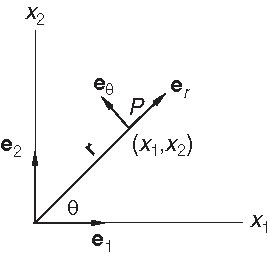
\includegraphics{../images/f02-33-01-H8560.jpg}
\caption{image}
\end{figure}
\end{columns}
\end{frame}

\begin{frame}{polar coordinates}
\protect\hypertarget{polar-coordinates-1}{}
\begin{columns}[T]
\textless div class=``column'' width=``50\%''

\begin{figure}
\centering
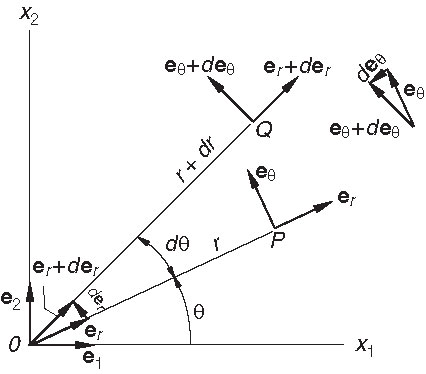
\includegraphics{../images/f02-33-02-H8560.jpg}
\caption{image}
\end{figure}
\end{columns}
\end{frame}

\begin{frame}{polar coordinates}
\protect\hypertarget{polar-coordinates-2}{}
\begin{itemize}
\tightlist
\item
  We can now find the components of \(\nabla f\), \(\nabla v_i\),
  \(\text{div} (v_i)\), \(\text{div} (T_{ij})\), \(\nabla^2f\) and
  \(\nabla^2 v_i\).
  \[\nabla f = \langle f_{,r}, \frac{1}{r}f_{,\theta} \rangle\]
\end{itemize}

\[= \begin{bmatrix}
    v_{r,r} & \frac{1}{r}(v_{r,\theta}-v_\theta)\\
    v_{\theta,r} & \frac{1}{r}(v_{\theta,\theta}-v_r)
\end{bmatrix}\]

\[\text{div} (v_i) = \text{tr} (\nabla v_i) = v_{r,r} +\frac{1}{r}(v_{\theta,\theta}+v_r)\]
\end{frame}

\begin{frame}{polar coordinates}
\protect\hypertarget{polar-coordinates-3}{}
\[\text{curl} (v_i) = \langle 0, 0, v_{\theta,r} + \frac{v_\theta}{r} - \frac{1}{r}v_{r,\theta} \rangle\]

\[\text{div} (T_{ij}) = \langle T_{rr,r} + \frac{1}{r}T_{r\theta,\theta} + \frac{T_{rr}-T_{\theta\theta}}{r}, T_{r\theta,r} + \frac{1}{r} T_{\theta\theta,\theta} + \frac{T_{r\theta} + T_{\theta r}}{r} \rangle\]

\[\nabla^2 f = f_{,rr} + \frac{1}{r^2} f_{,\theta\theta} + \frac{1}{r}f_{,r}\]

\[\begin{aligned}
    \nabla^2 v_i =& \langle v_{r,rr} + \frac{1}{r^2}v_{r,\theta\theta} + v_{r,zz} + \frac{1}{r}v_{r,r} - \frac{2}{r^2}v_{\theta,\theta}-\frac{v_r}{r^2},\\
    & v_{\theta,rr} + \frac{1}{r^2}v_{\theta,\theta\theta} + \frac{1}{r}v_{\theta,r} + \frac{2}{r^2}v_{r,\theta}- \frac{v_\theta}{r^2}\rangle
\end{aligned}\]
\end{frame}

\begin{frame}{cylindrical coordinates}
\protect\hypertarget{cylindrical-coordinates}{}
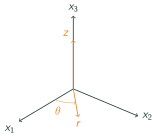
\includegraphics{../images/cylindrical.svg}
\end{frame}

\begin{frame}{cylindrical coordinates}
\protect\hypertarget{cylindrical-coordinates-1}{}
\begin{itemize}
\tightlist
\item
  Calculus in cylindrical coordinates is nearly identical to polar
  coordinates
\end{itemize}

\[\nabla f = \langle f_{,r}, \frac{1}{r}f_{,\theta}, f_{,z} \rangle\]

\[= \begin{bmatrix}
    v_{r,r} & \frac{1}{r}(v_{r,\theta}-v_\theta) & v_{r,z}\\
    v_{\theta,r} & \frac{1}{r}(v_{\theta,\theta}+v_r) & v_{\theta,z}\\
    v_{z,r} & \frac{v_{z,\theta}}{r} & v_{z,z}
\end{bmatrix}\]

\[\text{div} (v_i) = \text{tr} (\nabla v_i) = v_{r,r} +\frac{1}{r}(v_{\theta,\theta}+v_r) + v_{z,z}\]
\end{frame}

\begin{frame}{cylindrical coordinates}
\protect\hypertarget{cylindrical-coordinates-2}{}
\[\begin{aligned}
    \text{curl} (v_i) = \langle &\frac{v_{z,\theta}}{r} - v_{\theta,z},\\
    & v_{r,z} - v_{z,r},\\
    & v_{\theta,r} + \frac{v_\theta}{r} - \frac{v_{r,\theta}}{r} \rangle
\end{aligned}\]

\[\begin{aligned}
    \text{div} (T_{ij}) = \langle &T_{rr,r} + \frac{T_{r\theta,\theta}}{r} + \frac{T_{rr}-T_{\theta\theta}}{r} + T_{rz,z},\\
    &T_{r\theta,r} + \frac{T_{\theta\theta,\theta}}{r}  + \frac{T_{r\theta} + T_{\theta r}}{r} + T_{\theta z, z},\\
    &T_{zr,r} + \frac{T_{z\theta,\theta}}{r} + T_{zz,z} + T_{zr,r}\rangle
\end{aligned}\]

\[\nabla^2 f = f_{,rr} + \frac{1}{r^2} f_{,\theta\theta} + \frac{1}{r}f_{,r} + f_{,zz}\]
\end{frame}

\begin{frame}{cylindrical coordinates}
\protect\hypertarget{cylindrical-coordinates-3}{}
\[\begin{aligned}
    \nabla^2 v_i =& \langle v_{r,rr} + \frac{1}{r^2}v_{r,\theta\theta} + v_{r,zz} + \frac{1}{r}v_{r,r} - \frac{2}{r^2}v_{\theta,\theta}-\frac{v_r}{r^2},\\
    & v_{\theta,rr} + \frac{1}{r^2}v_{\theta,\theta\theta} + v_{\theta,zz} + \frac{1}{r}v_{\theta,r} + \frac{2}{r^2}v_{r,\theta}- \frac{v_\theta}{r^2},\\
    & v_{z,rr} + \frac{v_{z,\theta\theta}}{r^2} + \frac{v_{z,r}}{r} + v_{z,zz}\rangle
\end{aligned}\]
\end{frame}

\begin{frame}{spherical coordinates}
\protect\hypertarget{spherical-coordinates}{}
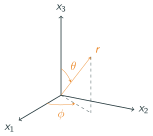
\includegraphics{../images/spheriical.svg}
\end{frame}

\begin{frame}{spherical coordinates}
\protect\hypertarget{spherical-coordinates-1}{}
\begin{itemize}
\tightlist
\item
  For calculus in spherical coordinates, we have
  \[\nabla f = \langle f_{,r}, \frac{f_{,\theta}}{r}, \frac{f_{,\phi}}{r \sin \theta} \rangle\]
\end{itemize}

\[\nabla v_i = \begin{bmatrix}
    v_{r,r} & \frac{v_{r,\theta}-v_\theta}{r} & \frac{v_{r,\phi}}{r \sin \theta} - \frac{v_\phi}{r}\\
    v_{\theta,r} & \frac{v_{\theta,\theta}+v_r}{r} & \frac{v_{\theta,\phi}}{r \sin \theta} - \frac{v_\phi \cot \theta}{r}\\
    v_{\phi,r} & \frac{v_{\phi,\theta}}{r} & \frac{v_{\phi,\phi}}{r\sin \theta} + \frac{v_r + v_\theta \cot \theta}{r}
\end{bmatrix}\]

\[\text{div} ( v_i) = \frac{(r^2v_r)_{,r}}{r^2} + \frac{(v_\theta \sin \theta)_{,\theta}}{r\sin \theta} + \frac{v_{\phi,\phi}}{r\sin\theta}\]
\end{frame}

\begin{frame}{spherical coordinates}
\protect\hypertarget{spherical-coordinates-2}{}
\[\text{curl} (v_i) = \langle \frac{v_\phi cot\theta+v_{\phi,\theta}}{r} - \frac{v_{\theta,\phi}}{r \sin \theta}, \frac{v_{r,\phi}}{r\sin\theta} - \frac{(rv_{\phi})_{,r}}{r}, \frac{(rv_\theta)_{,r}-v_{r,\theta}}{r} \rangle\]

\[\text{div}(T_{ij}) = \begin{aligned}\langle
    & \frac{(r^2T_{rr})_{,r}}{r^2} + \frac{(T_{r\theta}\sin\theta)_{,\theta}+T_{r\phi,\phi}}{r\sin\theta} - \frac{T_{\theta\theta} + T_{\phi\phi}}{r}\\
    & \frac{(r^3T_{\theta r})_{,r}}{r^3} + \frac{(T_{\theta\theta}\sin\theta)_{,\theta}+T_{\theta\phi,\phi}}{r\sin\theta} + \frac{T_{r\theta} - T_{\theta r}- T_{\phi\phi}\cot\theta}{r}\\
    & \frac{(r^3T_{\phi r})_{,r}}{r^3} + \frac{(T_{\phi\theta}\sin\theta)_{,\theta}+T_{\phi\phi,\phi}}{r\sin\theta} + \frac{T_{r\phi} - T_{\phi r}+ T_{\theta\phi}\cot\theta}{r}
\rangle\end{aligned}\]
\end{frame}

\begin{frame}{spherical coordinates}
\protect\hypertarget{spherical-coordinates-3}{}
\[\nabla^2 f = f_{,rr} + \frac{2 f_{,r}}{r} + \frac{f_{,\theta\theta}+ f_{,\theta}\cot \theta}{r^2} + \frac{f_{,\phi \phi}}{r^2\sin^2\theta}\]

\[\nabla^2 v_i = \begin{aligned}
    \langle & \frac{(r^2v_r)_{,rr}+v_{r,\theta\theta} + v_{r,\theta}\cot \theta}{r^2} - \frac{2(r^2v_r)_{,r}}{r^3} + \frac{v_{r,\phi \phi}}{r^2\sin^2\theta} \\
    &\qquad - \frac{2(v_\theta \sin \theta)_{,\theta} + 2v_{\phi,\phi}}{r^2 \sin \theta}\\
    &\frac{(r^2 v_{\theta,r})_{,r} \left(\frac{(v_{\theta}\sin\theta)_{,\theta}}{\sin \theta}\right)_{,\theta} + 2v_{r,\theta}}{r^2} + \frac{v_{\theta,\phi\phi}}{r^2\sin^2\theta} - \frac{2 \cot \theta v_{\phi,\phi}}{r^2 \sin\theta}\\
    &\frac{(r^2 v_{\phi,r})_{,r} \left(\frac{(v_{\phi}\sin\theta)_{,\theta}}{\sin \theta}\right)_{,\theta}}{r^2} + \frac{v_{\phi,\phi\phi}}{r^2\sin^2\theta} + \frac{2v_{r,\phi} + 2 \cot \theta v_{\theta,\phi}}{r^2 \sin\theta}
\rangle \end{aligned}\]
\end{frame}

\begin{frame}{spherical coordinates}
\protect\hypertarget{spherical-coordinates-4}{}
\begin{itemize}
\tightlist
\item
  Calculate \(\text{div}(u_i)\) in spherical coordinates for the vector
  field
\end{itemize}

\[u_i = \langle Ar + \frac{B}{r^2}, 0, 0 \rangle\]
\end{frame}

\begin{frame}{group one}
\protect\hypertarget{group-one}{}
\begin{itemize}
\item
  Solve the following expression for \(T_{ij}\)
  \[E_{ij} = \frac{1}{2\mu} \left[T_{ij} - \frac{\lambda}{3\lambda + 2\mu} T_{kk} \delta_{ij}\right]\]
\item
  Hint: First solve for \(T_{kk}\), and then substitute that result to
  complete the solution
\end{itemize}
\end{frame}

\begin{frame}{group two}
\protect\hypertarget{group-two}{}
\begin{itemize}
\item
  For the tensor \(T_{ij}\), \[T_{ji} = \begin{bmatrix}
  1& 5 & -5\\
  5 & 0 & 0\\
    -5 & 0 & 1
  \end{bmatrix}\] find \(T_{11}^\prime\) where
  \(e_1^\prime = -e_2 + 2e_3\) and \(e_2^\prime = e_1\)
\item
  Hint: unless you have an advanced calculator, this problem will be
  easier in tensor notation, since you need only find one term of the
  transformed tensor (let \(i=j=1\)).
\end{itemize}
\end{frame}

\begin{frame}{group three}
\protect\hypertarget{group-three}{}
\begin{itemize}
\item
  Consider the ellipsoidal surface defined by
  \[\frac{x^2}{a^2} + \frac{y^2}{b^2} + \frac{z^2}{b^2} = 1\]
\item
  Find the unit vector normal to the surface at some point, \((x,y,z)\)
\end{itemize}
\end{frame}

\begin{frame}{group four}
\protect\hypertarget{group-four}{}
\begin{itemize}
\tightlist
\item
  Calculate \(\text{div}(u_i)\) in cylindrical coordinates for the
  vector field \[u_i = \langle \frac{\sin \theta}{r}, 0, 0 \rangle\]
\end{itemize}
\end{frame}
